\section{MAPE-K Loop }
The MAPE-K loop first proposed by IBM is one of the most popular feedback loops which is used to allocate resources and diagnose the failures during runtime in self adaptive systems. The feedback loop comprises of four phases: monitor, analyse, plan, execute with knowledge, together referred to as MAPE-K loop. Figure 0.1 shows the different components of the MAPE-K loop which we will discuss in the subsequent section. In the mapek autonomic control loop, managed resources are software or hardware components which are coupled with the autonomic manager to give autonomic behaviour to the reference model. Sensors are probes or gauges which collect information about the managed resources. Effectors change the behaviour of the managed system. Monitor collects information and data from the managed resources and filters them until a symptom is generated that needs to be analysed. Analyse performs data analysis depending on the symptoms generated by the monitor function. Plan selects the appropriate procedures to achieve goals and objectives. Execute carries out changes to the behaviour of the managed resources.


\begin{figure}[H]
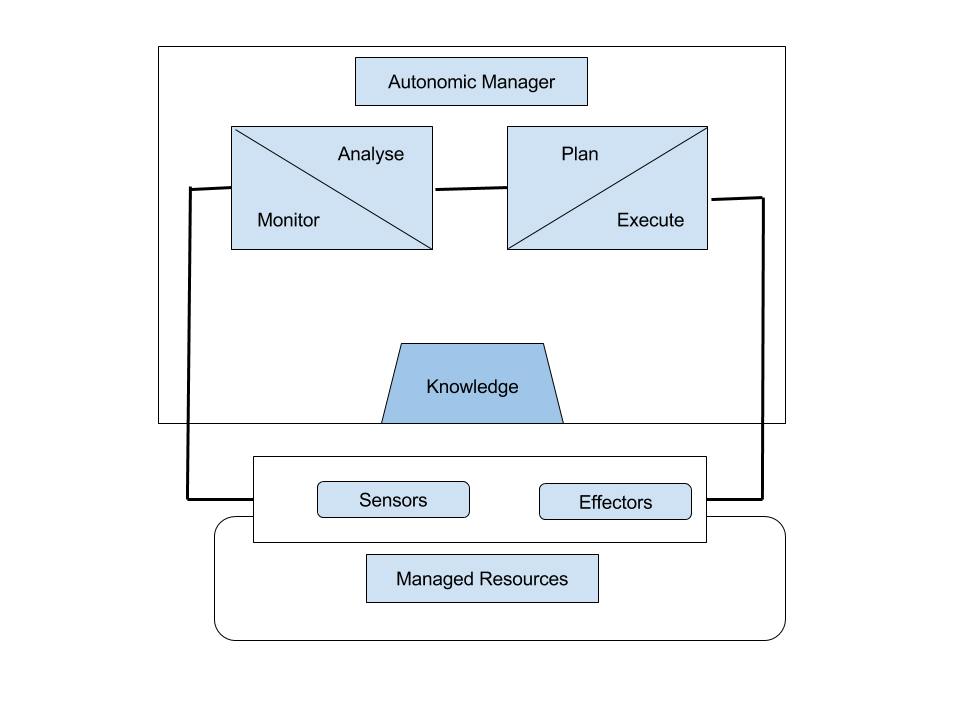
\includegraphics[width=5in]{img/ibmmapekloop}
\caption{IBM autonomic mapek loop}
\end{figure}
\paragraph*{Monitor}
The monitoring phase works in collaboration with the knowledge of the managed system. It collects data, information related to managed system and updates the knowledge accordingly. Prior to updating there is a preprocessing phase which filters the collected data. The monitor function aggregates these collected information after filtration and invokes the analyse phase once a symptom is identified that needs to be analysed.

\paragraph*{Analyse}

The analyse phase works in collaboration with the knowledge and the monitor phase and performs operations based on the symptoms provided by the monitoring phase.  
The analyse function compares and correlates the incoming data with the knowledge base to diagonise and analyse the symptoms. If adaptation actions are required based on the symptoms the trigger is passed to the plan phase. 
 

\paragraph*{Plan}

Once the analyse phase is completed the plan is triggered which selects the procedure
to be adapted by the managed system when adaptation plans are required. Depending on the analyse phase the planning is done. No adaptation plan is required when system is satisfied. 


\paragraph*{Execute}

The execute phase works using the effectors for changing the behaviour of the managed
system based on the adaptation actions recommended by the plan phase.The execute behaviour performs the preparation task before executing the actions for addition of the resources to the system. The preparation tasks include locking of certain resources keeping the system in safe state. After the
execution is complete, the plan is checked for its completion. If some actions remain pending, the process is repeated for next actions to the managed resources.

\paragraph*{Knowledge}

The knowledge of the managed system shares data among each of the components of
the MAPE-K loop. The shared knowledge contains information about the managed system
knowledge which includes data such as resource types, number of resources, historical
logs and metrics. The knowledge function is created by the monitoring phase and the
execute phase updates the knowledge accordingly while consulting the plan function. 
\cite{kephart2003vision}.\\


